\documentclass[11pt,a4paper]{article}

\usepackage[utf8]{inputenc}
\usepackage[T1]{fontenc}
\usepackage[italian]{babel}
\usepackage{geometry}
\usepackage{graphicx}
\usepackage{hyperref}
\usepackage{xcolor}
\usepackage{listings}
\usepackage{enumitem}
\usepackage{float}

\geometry{margin=2.5cm}
\graphicspath{{../images/}}

\hypersetup{
    colorlinks=true,
    linkcolor=black,
    urlcolor=blue
}

\lstdefinestyle{mesoscode}{
    basicstyle=\ttfamily\small,
    breaklines=true,
    frame=single,
    columns=fullflexible,
    keepspaces=true,
    showstringspaces=false
}
\lstdefinelanguage{json}{
    basicstyle=\ttfamily\small,
    morestring=[b]",
    stringstyle=\color{blue},
    morecomment=[l]{//},
    commentstyle=\color{gray},
    literate=
     *{0}{{{\color{black}0}}}{1}
      {1}{{{\color{black}1}}}{1}
      {2}{{{\color{black}2}}}{1}
      {3}{{{\color{black}3}}}{1}
      {4}{{{\color{black}4}}}{1}
      {5}{{{\color{black}5}}}{1}
      {6}{{{\color{black}6}}}{1}
      {7}{{{\color{black}7}}}{1}
      {8}{{{\color{black}8}}}{1}
      {9}{{{\color{black}9}}}{1}
      {:}{{{\color{black}{:}}}}{1}
      {,}{{{\color{black}{,}}}}{1}
      {\{}{{{\color{black}{\{}}}}{1}
      {\}}{{{\color{black}{\}}}}}{1}
      {[}{{{\color{black}{[}}}}{1}
      {]}{{{\color{black}{]}}}}{1}
}
\lstset{style=mesoscode}

\title{Protocollo di comunicazione client-server}
\author{Gruppo GC3}
\date{}

\begin{document}

\maketitle
\tableofcontents
\newpage

\section{Protocollo di comunicazione}

Il progetto adotta un'architettura MVC distribuita: view, controller e model si trovano in
processi diversi, quindi le interazioni devono necessariamente attraversare la rete.
Per mantenere una architettura e pulita, la rete deve essere
trasparente per la logica applicativa: né la view né il model ne il controller 
devono sapere se stanno comunicando via TCP o RMI, per loro deve essere come se si trovino
sulla stessa macchina.

Per raggiungere questo obiettivo il sistema introduce due contratti che simulano localmente
la presenza della controparte remota --- ciascuno finge di essere l'oggetto che il proprio
lato dovrebbe avere vicino:
\begin{itemize}
    \item \texttt{VirtualView} (risiede sul server): per il model è la view del client.
    Il model la registra come listener tramite l'Observer pattern e chiama
    \texttt{notifyUpdate()} su di essa esattamente come farebbe con una view locale;
    è la \texttt{VirtualView} concreta che si occupa di serializzare e trasportare
    l'aggiornamento attraverso la rete verso il client reale.

    \item \texttt{VirtualServer} (risiede sul client): per la UI è il lato ricevente
    del server. Riceve i messaggi che arrivano dalla rete e li consegna alla view locale,
    che non sa nulla del trasporto sottostante.
\end{itemize}

Questi contratti hanno un doppio ruolo: a livello architetturale sono i punti di comunicazione
tra client e server; a livello implementativo permettono a TCP e RMI di offrire gli stessi
servizi funzionali, senza che la logica applicativa debba sapere quale protocollo è in uso.

Tuttavia, TCP e RMI hanno vincoli tecnici diversi che impediscono di usare le stesse interfacce
in entrambi i casi.
Nel caso TCP le interfacce sono normali interfacce Java.
Nel caso RMI, invece, le interfacce remote devono estendere \texttt{Remote} e i loro metodi
devono dichiarare \texttt{RemoteException}, perché RMI non può garantire che una chiamata
remota abbia successo come farebbe una chiamata locale.

Questa differenza introduce nel codice due livelli di contratto:
\begin{itemize}
    \item \textbf{Livello applicativo} --- \texttt{VirtualView} e \texttt{VirtualServer}
    descrivono i servizi indipendentemente dal protocollo usato;
    \item \textbf{Livello RMI} --- \texttt{RmiServerService} e \texttt{RmiClientService}
    espongono servizi equivalenti con i vincoli tecnici richiesti da RMI.
\end{itemize}

L'allineamento funzionale tra i due livelli è quindi:
\begin{itemize}
    \item \texttt{VirtualView} $\leftrightarrow$ \texttt{RmiServerService}: comandi client
    $\rightarrow$ server;
    \item \texttt{VirtualServer} $\leftrightarrow$ \texttt{RmiClientService}: notifiche server
    $\rightarrow$ client.
\end{itemize}

RMI richiede un ulteriore contratto, \texttt{RmiConnectionService}, che non ha un corrispondente
nel livello applicativo.
Viene usato dal client per aprire la connessione iniziale, ottenere lo stub della propria sessione
server-side e passare al server il proprio callback per le notifiche.
È il punto di ingresso di tutta la comunicazione RMI, prima che esistano sessioni individuali
per ogni client.

\section{Messaggi e payload usati dal protocollo}

Nel codice bisogna distinguere tra messaggio e payload.
Il payload contiene i dati applicativi veri e propri: il nickname scelto dal client,
l'id della lobby, la carta selezionata, lo stato aggiornato della partita.
Il messaggio è l'envelope che aggiunge le informazioni necessarie a interpretare quel payload.

La forma concreta che hanno questi tipi è dettata principalmente dal problema di TCP.
Sulla socket arriva solo una stringa JSON: il ricevente non sa a priori quale classe
concreta di payload ricostruire, perché a livello di contratto il payload è visto solo
tramite le interfacce \texttt{ClientPayload} o \texttt{ServerPayload}.
Per risolvere questo problema ogni messaggio include un campo \texttt{type}, che fa da
discriminante: il ricevente legge prima il tipo, poi chiede a GSON di deserializzare
il payload nella classe concreta corrispondente.

Il wrapper esiste quindi in due varianti, una per ciascuna direzione:
\begin{itemize}
    \item \texttt{ClientMessage}, con un \texttt{ClientMessageType} e un payload che
    implementa \texttt{ClientPayload}, per i messaggi client $\rightarrow$ server;
    \item \texttt{ServerMessage}, con un \texttt{ServerMessageType} e un payload che
    implementa \texttt{ServerPayload}, per i messaggi server $\rightarrow$ client.
\end{itemize}

RMI non ha questo problema: gli oggetti vengono passati direttamente tramite invocazione
remota, senza serializzazione JSON esplicita.
Tuttavia riutilizza gli stessi payload, così TCP e RMI condividono lo stesso contratto
dati a livello applicativo e la logica di dominio non dipende dal protocollo scelto.

I payload sono organizzati gerarchicamente rispetto alla fase di gioco:
\begin{itemize}
    \item pre-lobby: payload usati nella fase di autenticazione e scoperta delle lobby;
    \item lobby: payload usati nella fase di creazione e gestione della lobby;
    \item in-game: payload usati durante la partita.
\end{itemize}

E rispetto al senso di comunicazione:
\begin{itemize}
    \item client $\rightarrow$ server: package \texttt{clienttoserver}, 
    \texttt{ClientPayload};
    \item server $\rightarrow$ client: package \texttt{servertoclient}, 
    \texttt{ServerPayload}.
\end{itemize}

\begin{figure}[H]
    \centering
    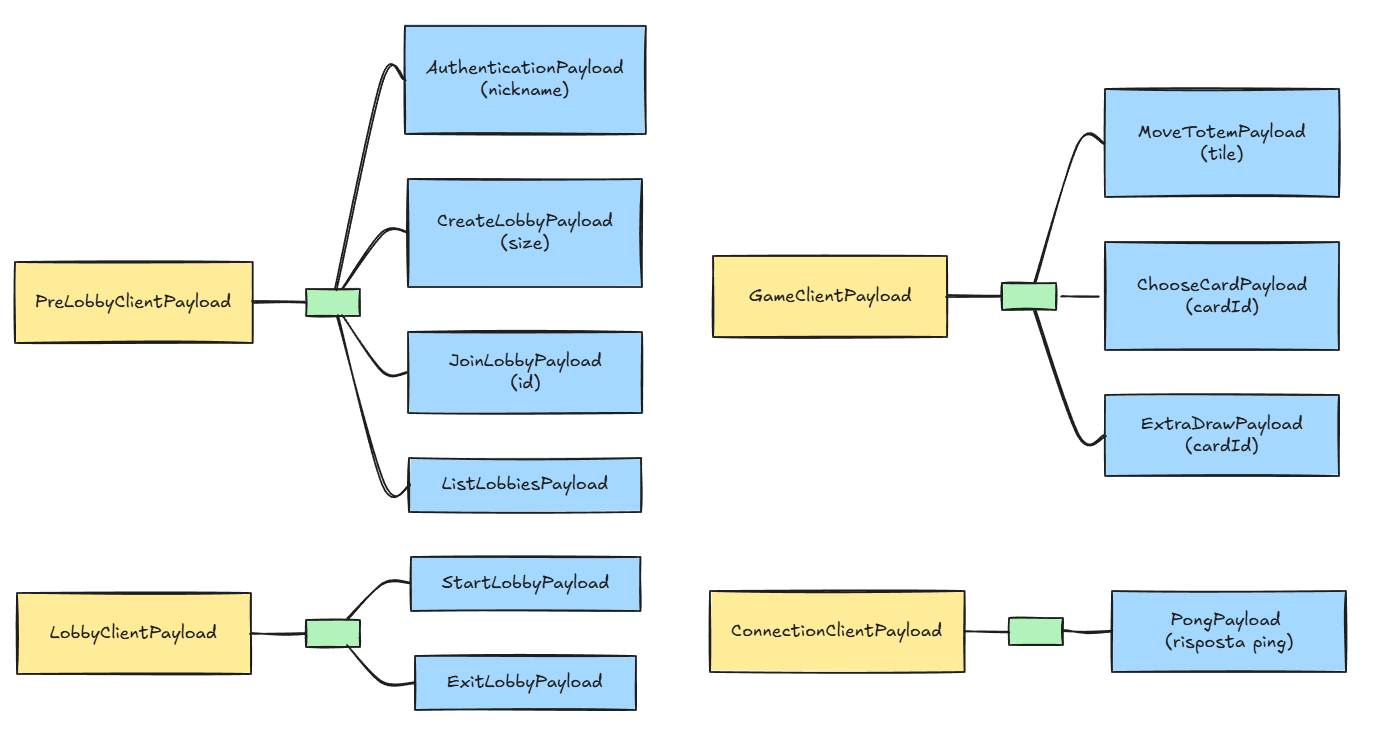
\includegraphics[width=\textwidth]{clientPayload.png}
    \caption{Gerarchia dei payload client $\rightarrow$ server}
\end{figure}

\begin{figure}[H]
    \centering
    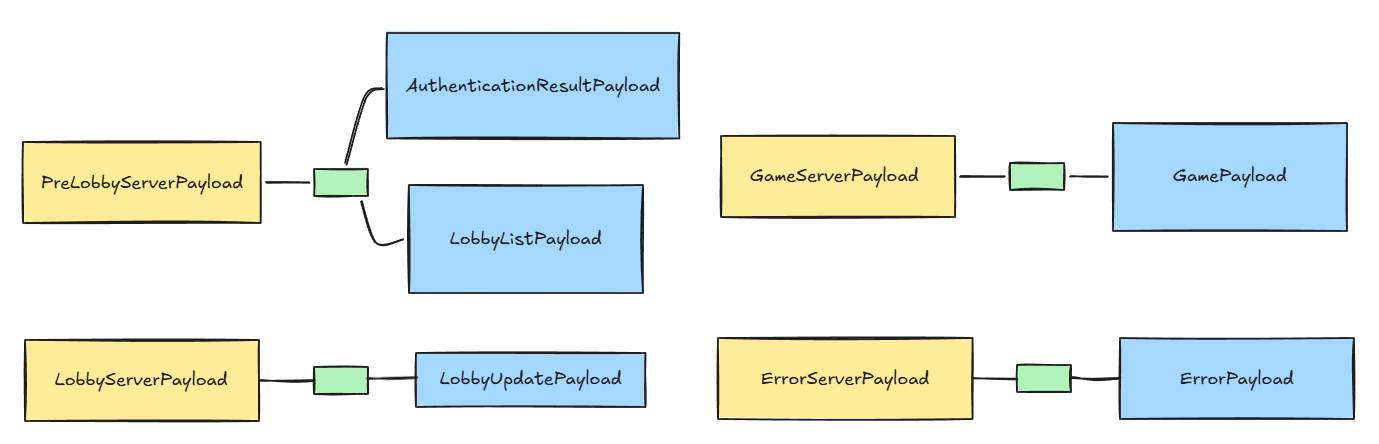
\includegraphics[width=\textwidth]{serverPayload.png}
    \caption{Gerarchia dei payload server $\rightarrow$ client}
\end{figure}

Alcuni payload, come \texttt{LobbySummaryPayload}, \texttt{BoardPayload},
\texttt{PlayerPayload}, \texttt{CardPayload}, \texttt{OfferSpacePayload},
\texttt{StartingBlockPayload}, \texttt{TribePayload}, \texttt{TurnOrderPayload} e
\texttt{TurnStatePayload}, non vengono inviati direttamente come messaggi principali
ma sono payload di supporto annidati dentro payload più grandi, usati per strutturare
dati complessi come lo stato della board o il turno corrente.

\section{Protocollo TCP}

TCP è un protocollo di trasporto che si basa su un canale di comunicazione bidirezionale:
la socket, identificata univocamente dalla quadrupla
\texttt{(IP\_sorgente, porta\_sorgente, IP\_destinazione, porta\_destinazione)}.
Una volta stabilita la connessione, i due endpoint possono scrivere e leggere dati
sullo stesso canale in entrambe le direzioni.

Dal punto di vista dei dati, però, la socket espone uno stream continuo di byte: non esiste
un confine naturale tra un messaggio e il successivo.
È quindi responsabilità dell'applicazione definire un protocollo di framing.
Nel progetto la scelta è semplice: ogni messaggio applicativo viene serializzato in JSON
e scritto sulla socket come una singola riga di testo.
Dall'altro lato il messaggio viene letto con \texttt{readLine()}, quindi una riga
corrisponde a un messaggio applicativo completo.

La lettura con \texttt{readLine()} è bloccante: il thread rimane sospeso finché non arriva
una riga completa o la connessione non si chiude.
Per questo motivo la lettura non può avvenire sul thread principale: sia il server che il
client dedicano un thread separato alla ricezione dei messaggi, così il resto
dell'applicazione può continuare a operare mentre il thread di lettura è in attesa.

\begin{lstlisting}[language=Java]
while ((message = reader.readLine()) != null) {
    handleMessage(message);
}
\end{lstlisting}

La scrittura avviene invece solo quando c'è un comando o una notifica da inviare,
quindi non richiede un thread dedicato:

\begin{lstlisting}[language=Java]
writer.println(serializedMessage);
\end{lstlisting}

\subsection{Flusso lato server}

Sul server viene creato un \texttt{ConnectionAcceptor}, che apre la \texttt{ServerSocket}
sulla porta configurata e gira su un thread dedicato in attesa di nuove connessioni:

\begin{lstlisting}[language=Java]
ConnectionAcceptor acceptor = new ConnectionAcceptor(tcpPort, serverConnectionLifecycle, router);
Thread acceptorThread = new Thread(acceptor, "mesos-connection-acceptor");
acceptorThread.start();
\end{lstlisting}

Per ogni client che si connette, il \texttt{ConnectionAcceptor} crea una
\texttt{VirtualViewTCP} dedicata e la avvia su un thread proprio:

\begin{lstlisting}[language=Java]
Socket clientSocket = this.serverSocket.accept();
VirtualViewTCP virtualView = new VirtualViewTCP(clientSocket, this.serverConnectionLifecycle, this.router);
Thread virtualViewThread = new Thread(virtualView, "mesos-virtual-view-" + clientSocket.getPort());
virtualViewThread.start();
\end{lstlisting}

Ogni \texttt{VirtualViewTCP} è quindi la sessione di un singolo client: gira sul proprio
thread, legge i messaggi in arrivo da quel client e può inviare notifiche verso di lui.

\subsection{Flusso lato client}

Sul client, \texttt{ServerProxyTCP} apre la socket verso il server e prepara il writer
per i messaggi in uscita.
Contestualmente avvia un \texttt{VirtualServerTCP} su un thread dedicato, che si occupa
di restare in ascolto dei messaggi in ingresso dal server:

\begin{lstlisting}[language=Java]
this.socket = new Socket(serverHost, port);
this.writer = new PrintWriter(this.socket.getOutputStream(), true);
this.virtualServer = new VirtualServerTCP(this.socket, clientView, this);
this.virtualServerThread = new Thread(this.virtualServer, "mesos-client-server-message-receiver");
this.virtualServerThread.start();
\end{lstlisting}

Dentro \texttt{VirtualServerTCP} viene preparato il reader e parte il ciclo di lettura:

\begin{lstlisting}[language=Java]
BufferedReader reader = new BufferedReader(new InputStreamReader(this.socket.getInputStream()));

while (this.running && (serializedMessage = reader.readLine()) != null) {
    this.handleMessage(serializedMessage);
}
\end{lstlisting}

\begin{figure}[H]
    \centering
    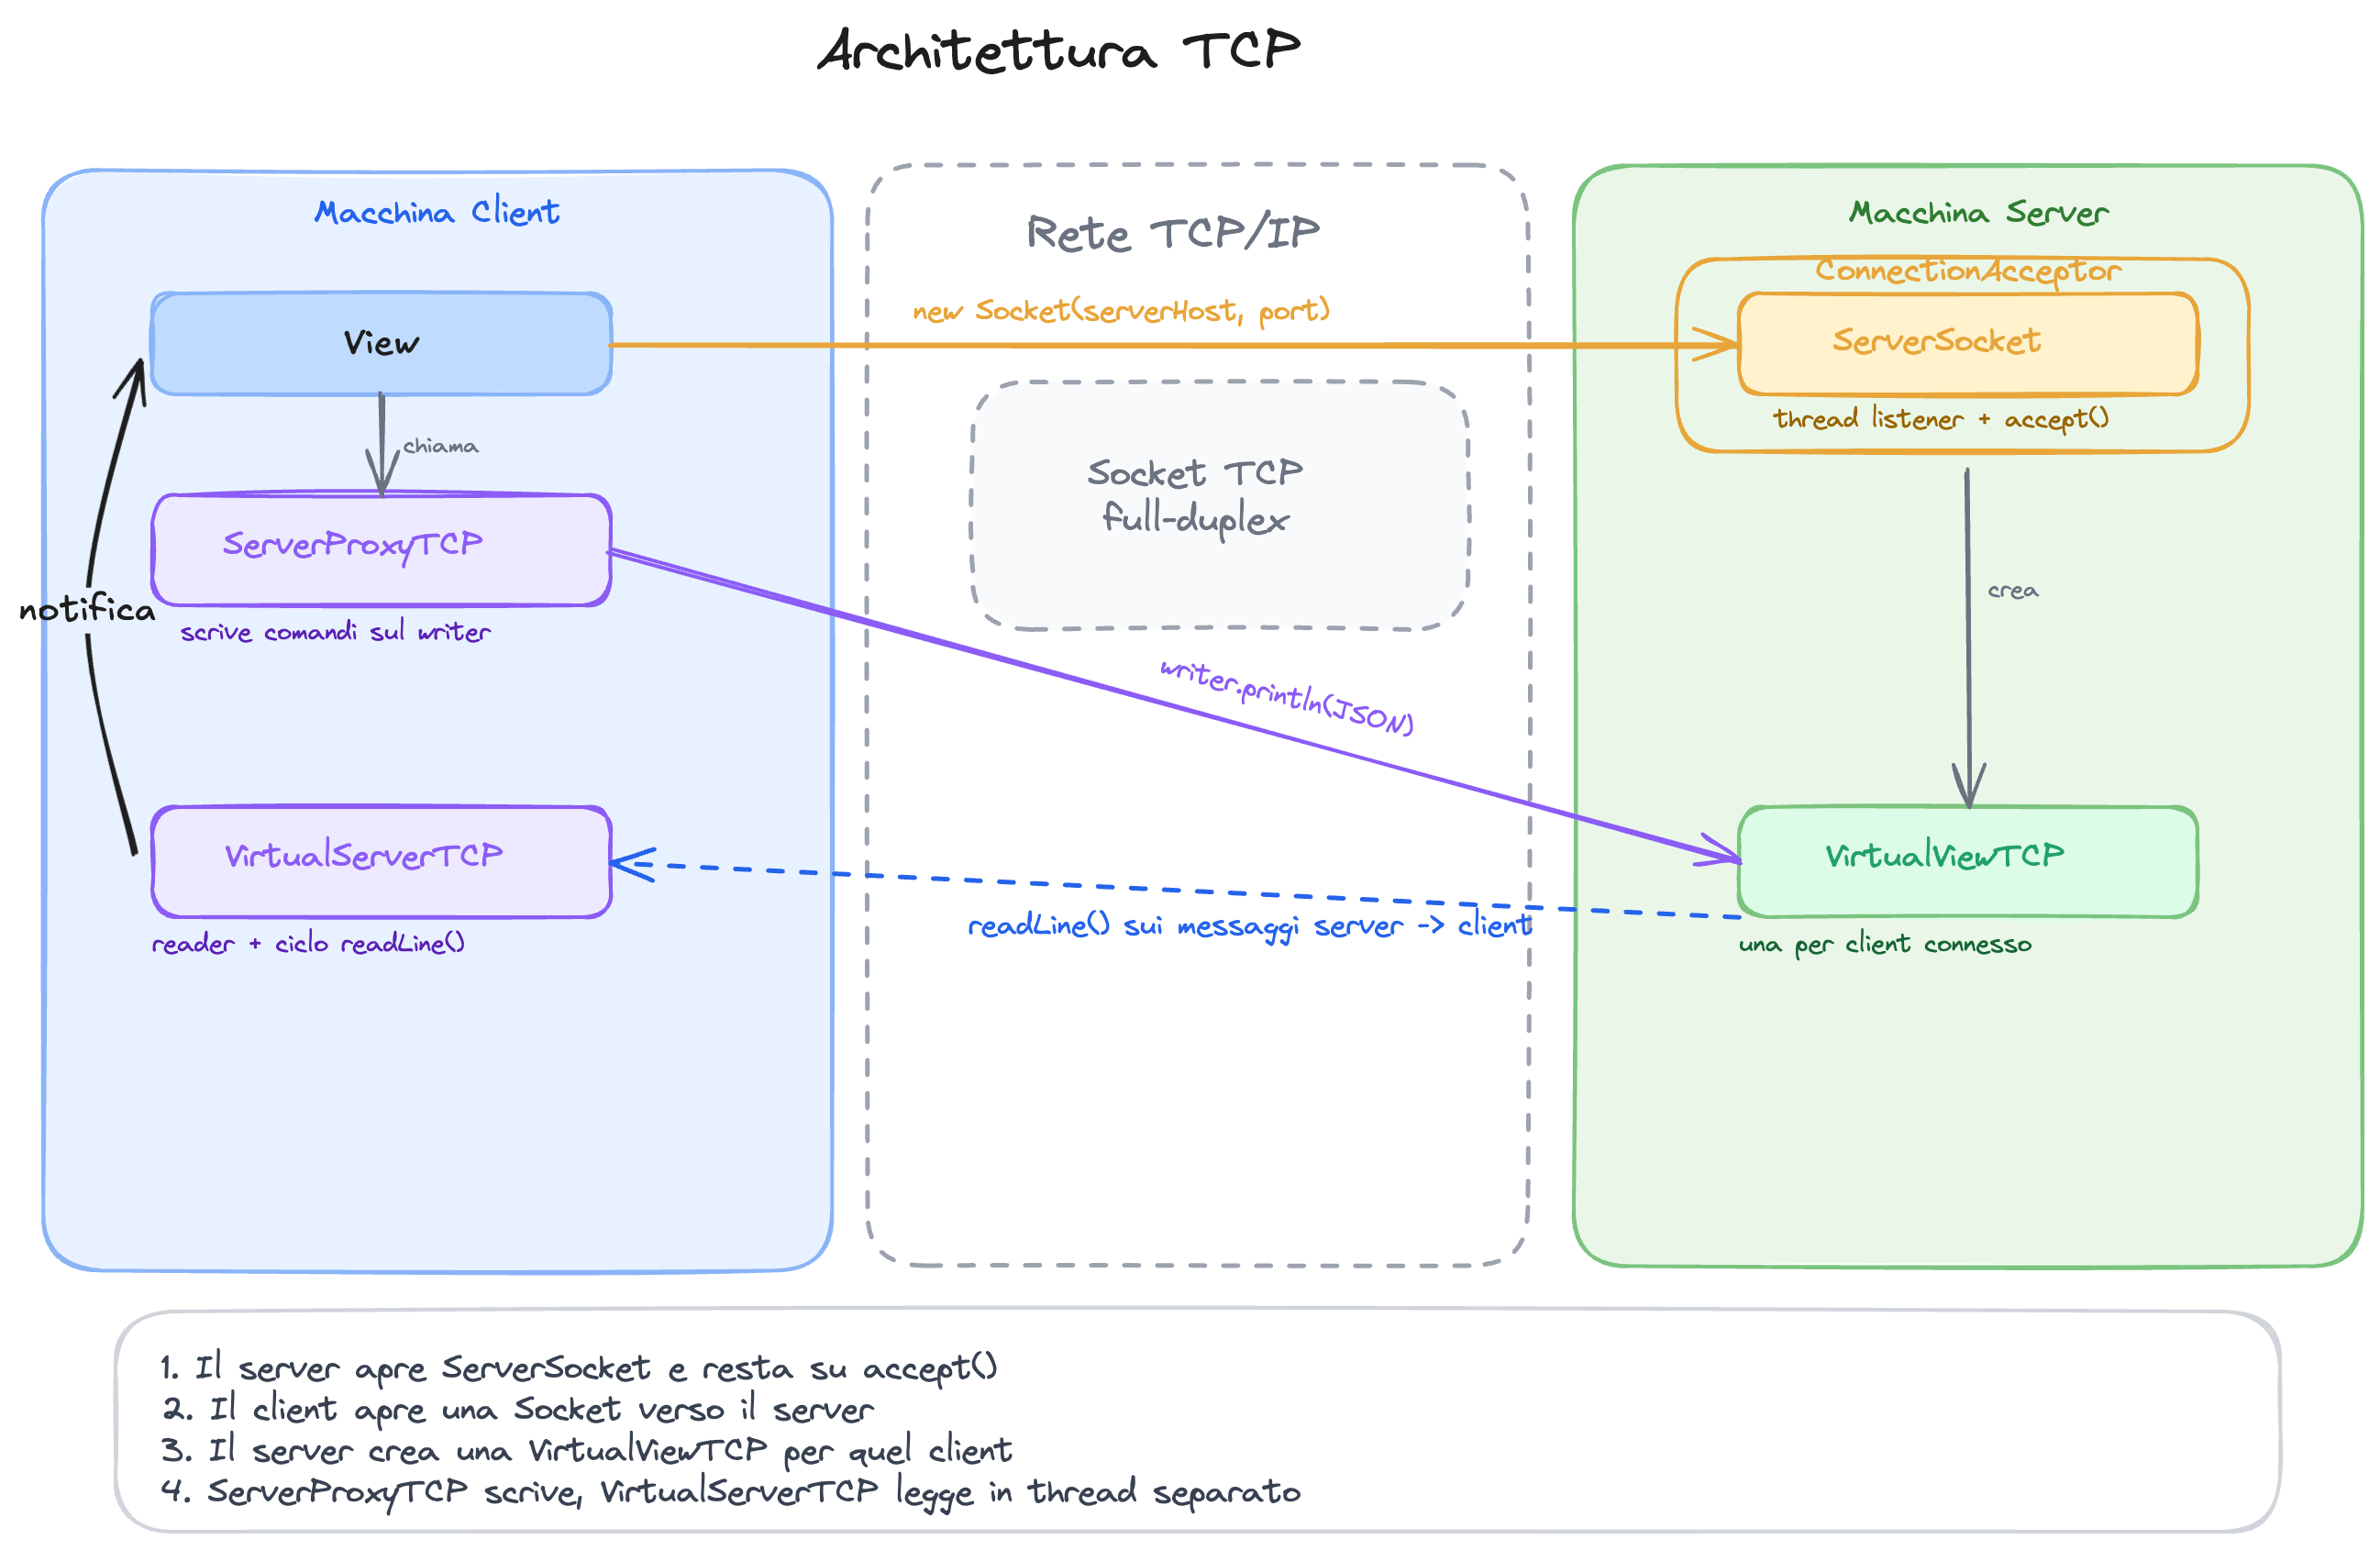
\includegraphics[width=\textwidth]{FlussoTCP.png}
    \caption{Flusso TCP}
\end{figure}

In sintesi il flusso concreto TCP è:
\begin{itemize}
    \item il server avvia il \texttt{ConnectionAcceptor} su un thread dedicato;
    \item per ogni client che si connette viene creata una \texttt{VirtualViewTCP}
    su un proprio thread;
    \item il client apre la socket e avvia \texttt{VirtualServerTCP} su un thread
    dedicato alla ricezione;
    \item client $\rightarrow$ server: \texttt{ServerProxyTCP} serializza e scrive
    sul writer;
    \item server $\rightarrow$ client: \texttt{VirtualViewTCP} serializza e scrive,
    \texttt{VirtualServerTCP} legge e consegna alla view.
\end{itemize}

\subsection{GSON}

GSON è la libreria usata per trasformare oggetti Java in stringhe JSON e viceversa.
La serializzazione di un messaggio in uscita è diretta:

\begin{lstlisting}[language=Java]
ClientMessage message = new ClientMessage(ClientMessageType.AUTHENTICATE, new AuthenticationPayload("tom"));
String serializedMessage = GSON.toJson(message);
\end{lstlisting}

La deserializzazione in ingresso è più articolata perché il campo \texttt{payload} è
dichiarato come interfaccia (\texttt{ClientPayload} o \texttt{ServerPayload}) e GSON
non sa quale classe concreta istanziare.
Il \texttt{type} fa quindi da discriminante: il messaggio viene prima letto come
\texttt{JsonObject} per estrarre il tipo, poi il payload viene deserializzato nella
classe concreta corrispondente.
Questo processo è visibile nel \texttt{ClientCommandHandler} lato server:

\begin{lstlisting}[language=Java]
JsonObject root = GSON.fromJson(rawMessage, JsonObject.class);
ClientMessageType type = ClientMessageType.valueOf(root.get("type").getAsString());
JsonElement payloadElement = root.get("payload");

ClientPayload payload = switch (type) {
    case AUTHENTICATE -> GSON.fromJson(payloadElement, AuthenticationPayload.class);
    case CREATE_LOBBY  -> GSON.fromJson(payloadElement, CreateLobbyPayload.class);
    case MOVE_TOTEM   -> GSON.fromJson(payloadElement, MoveTotemPayload.class);
    // altri type mappati sulle rispettive classi di payload
};
\end{lstlisting}

\section{Protocollo RMI}

RMI è un'astrazione Java per la comunicazione distribuita: permette a una JVM di invocare metodi
su oggetti che risiedono in un'altra JVM, con la stessa sintassi di una chiamata locale.
A differenza di TCP, il codice applicativo non apre socket, non serializza righe JSON e non mantiene
cicli di \texttt{readLine()}: questi aspetti restano presenti a livello di trasporto ma sono
nascosti dal meccanismo degli stub e delle interfacce remote.

La differenza architetturale rispetto a TCP riguarda soprattutto la direzione server
$\rightarrow$ client.
In TCP il server può scrivere al client in qualsiasi momento perché lo stream bidirezionale è
sempre aperto.
In RMI non esiste uno stream: tutto è invocazione di metodi su oggetti remoti.
Per notificare il client, il server ha bisogno di qualcosa da poter chiamare: per questo il client
deve esportare un oggetto remoto, la callback, e passarlo al server durante la connessione.

\begin{figure}[H]
    \centering
    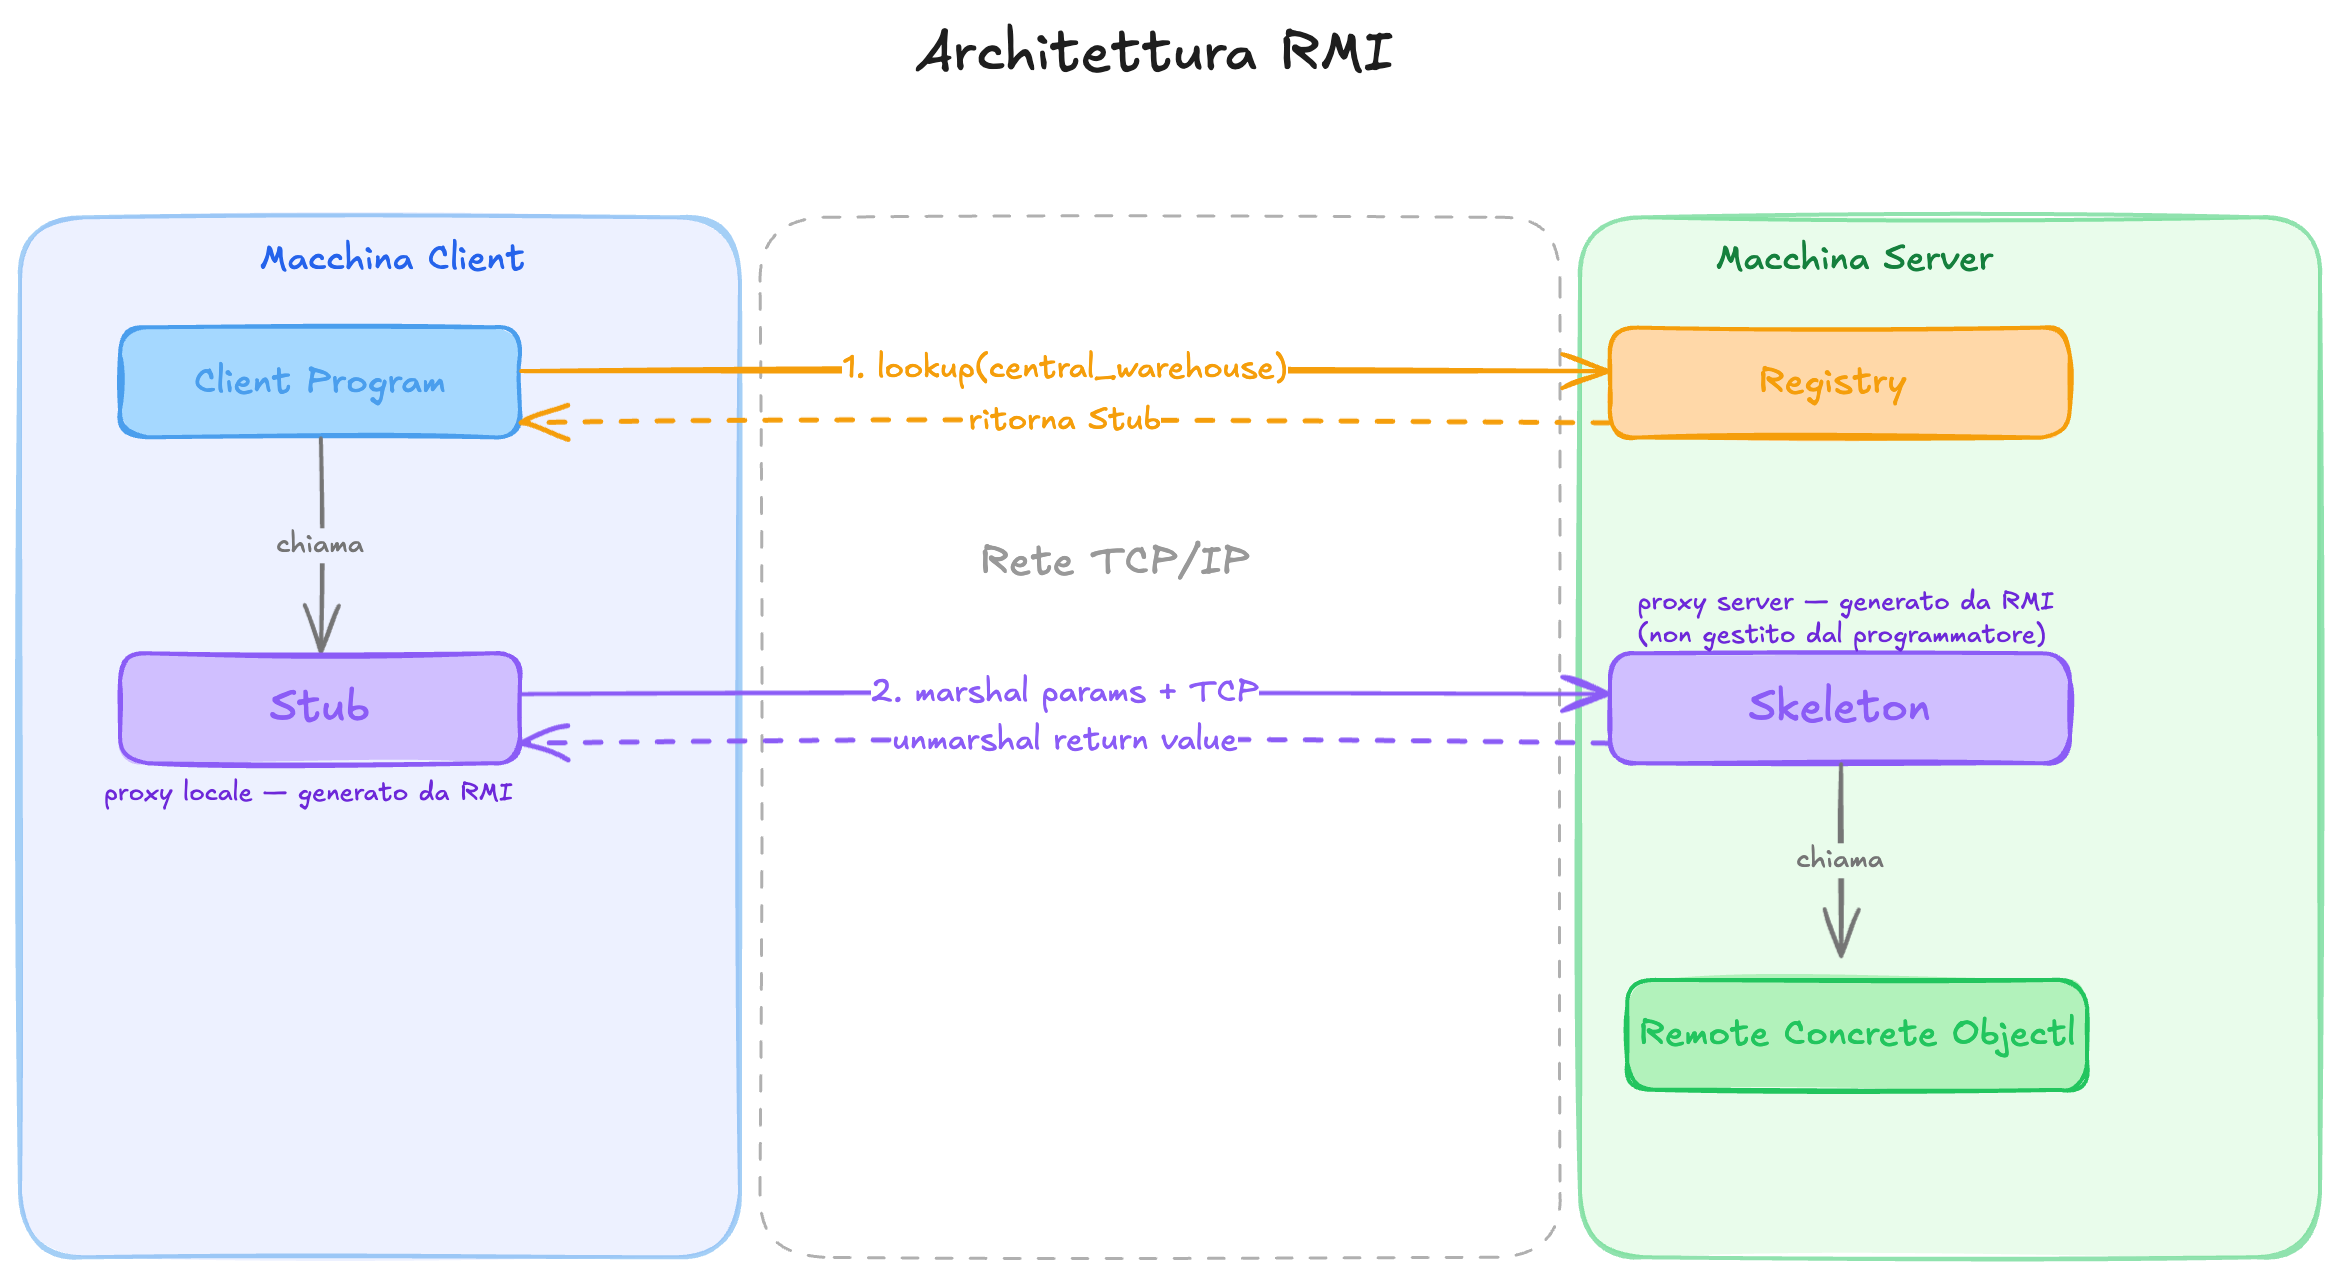
\includegraphics[width=\textwidth]{HighLevelRMI.png}
    \caption{Architettura RMI ad alto livello}
\end{figure}

\subsection{Setup Connessione}

Il server pubblica nel registry RMI un oggetto di tipo \texttt{RmiConnectionEntryPoint},
che implementa \texttt{RmiConnectionService} e viene registrato con il nome \texttt{MesosServer}.
Il registry funge da name service: permette al client di scoprire l'entry point del server
senza dover conoscere lo stub direttamente.

\begin{lstlisting}[language=Java]
RmiConnectionService rmiEntryPoint = new RmiConnectionEntryPoint(controller, router);
LocateRegistry.createRegistry(port);
Registry registry = LocateRegistry.getRegistry(port);
registry.rebind("MesosServer", rmiEntryPoint);
\end{lstlisting}

Il client ottiene lo stub dell'entry point tramite lookup:

\begin{lstlisting}[language=Java]
String registryUrl = "rmi://" + serverHost + ":" + rmiPort + "/MesosServer";
RmiConnectionService connectionService =
        (RmiConnectionService) Naming.lookup(registryUrl);
\end{lstlisting}

Prima di chiamare \texttt{connect(...)}, il client esporta il proprio callback RMI,
\texttt{VirtualServerRMI}: è l'oggetto remoto che il server chiamerà per consegnare
notifiche al client.

\begin{lstlisting}[language=Java]
this.callbackReceiver = new VirtualServerRMI(clientView, exportCallback);
this.serverStub = connectionService.connect(this.callbackReceiver);
this.callbackReceiver.attachServerProxy(this);
\end{lstlisting}

La chiamata a \texttt{connect(...)} arriva sul server in \texttt{RmiConnectionEntryPoint},
che riceve il callback e crea una \texttt{VirtualViewRMI} dedicata a quella sessione:

\begin{lstlisting}[language=Java]
public RmiServerService connect(RmiClientService clientCallback) throws RemoteException {
    return new VirtualViewRMI(this.serverConnectionLifecycle, clientCallback, this.router);
}
\end{lstlisting}

\texttt{VirtualViewRMI} è la sessione remota del singolo client lato server: registra la
connessione e conserva il callback ricevuto.

\begin{lstlisting}[language=Java]
this.clientCallback = clientCallback;
this.sessionId = this.serverConnectionLifecycle.registerConnection(this);
\end{lstlisting}

Il valore restituito da \texttt{connect(...)} è uno stub di tipo \texttt{RmiServerService},
che il client userà d'ora in poi per inviare comandi — senza più passare dal registry.

\subsection{Scambio messaggi}

Client $\rightarrow$ server: \texttt{ServerProxyRMI} invoca un metodo sullo stub
\texttt{RmiServerService}, la chiamata arriva in \texttt{VirtualViewRMI.handleClientMessage(...)}.
Il messaggio viene ricevuto come oggetto Java e inoltrato direttamente al router applicativo:

\begin{lstlisting}[language=Java]
this.serverStub.handleClientMessage(message);
\end{lstlisting}

\begin{lstlisting}[language=Java]
ClientPayload payload = clientMessage.payload;
this.router.routeMessage(this.sessionId, payload);
\end{lstlisting}

Server $\rightarrow$ client: il model notifica \texttt{VirtualViewRMI} tramite l'Observer pattern.
\texttt{VirtualViewRMI} invoca il metodo sul callback remoto del client:

\begin{lstlisting}[language=Java]
this.clientCallback.handleMessage(
        new ServerMessage(ServerMessageType.AUTHENTICATION_RESULT, authenticationResultPayload)
);
\end{lstlisting}

La chiamata arriva in \texttt{VirtualServerRMI.handleMessage(...)}, che la inoltra al
\texttt{MessageRouter} della UI:

\begin{lstlisting}[language=Java]
this.messageRouter.routeMessage(message);
\end{lstlisting}

\begin{figure}[H]
    \centering
    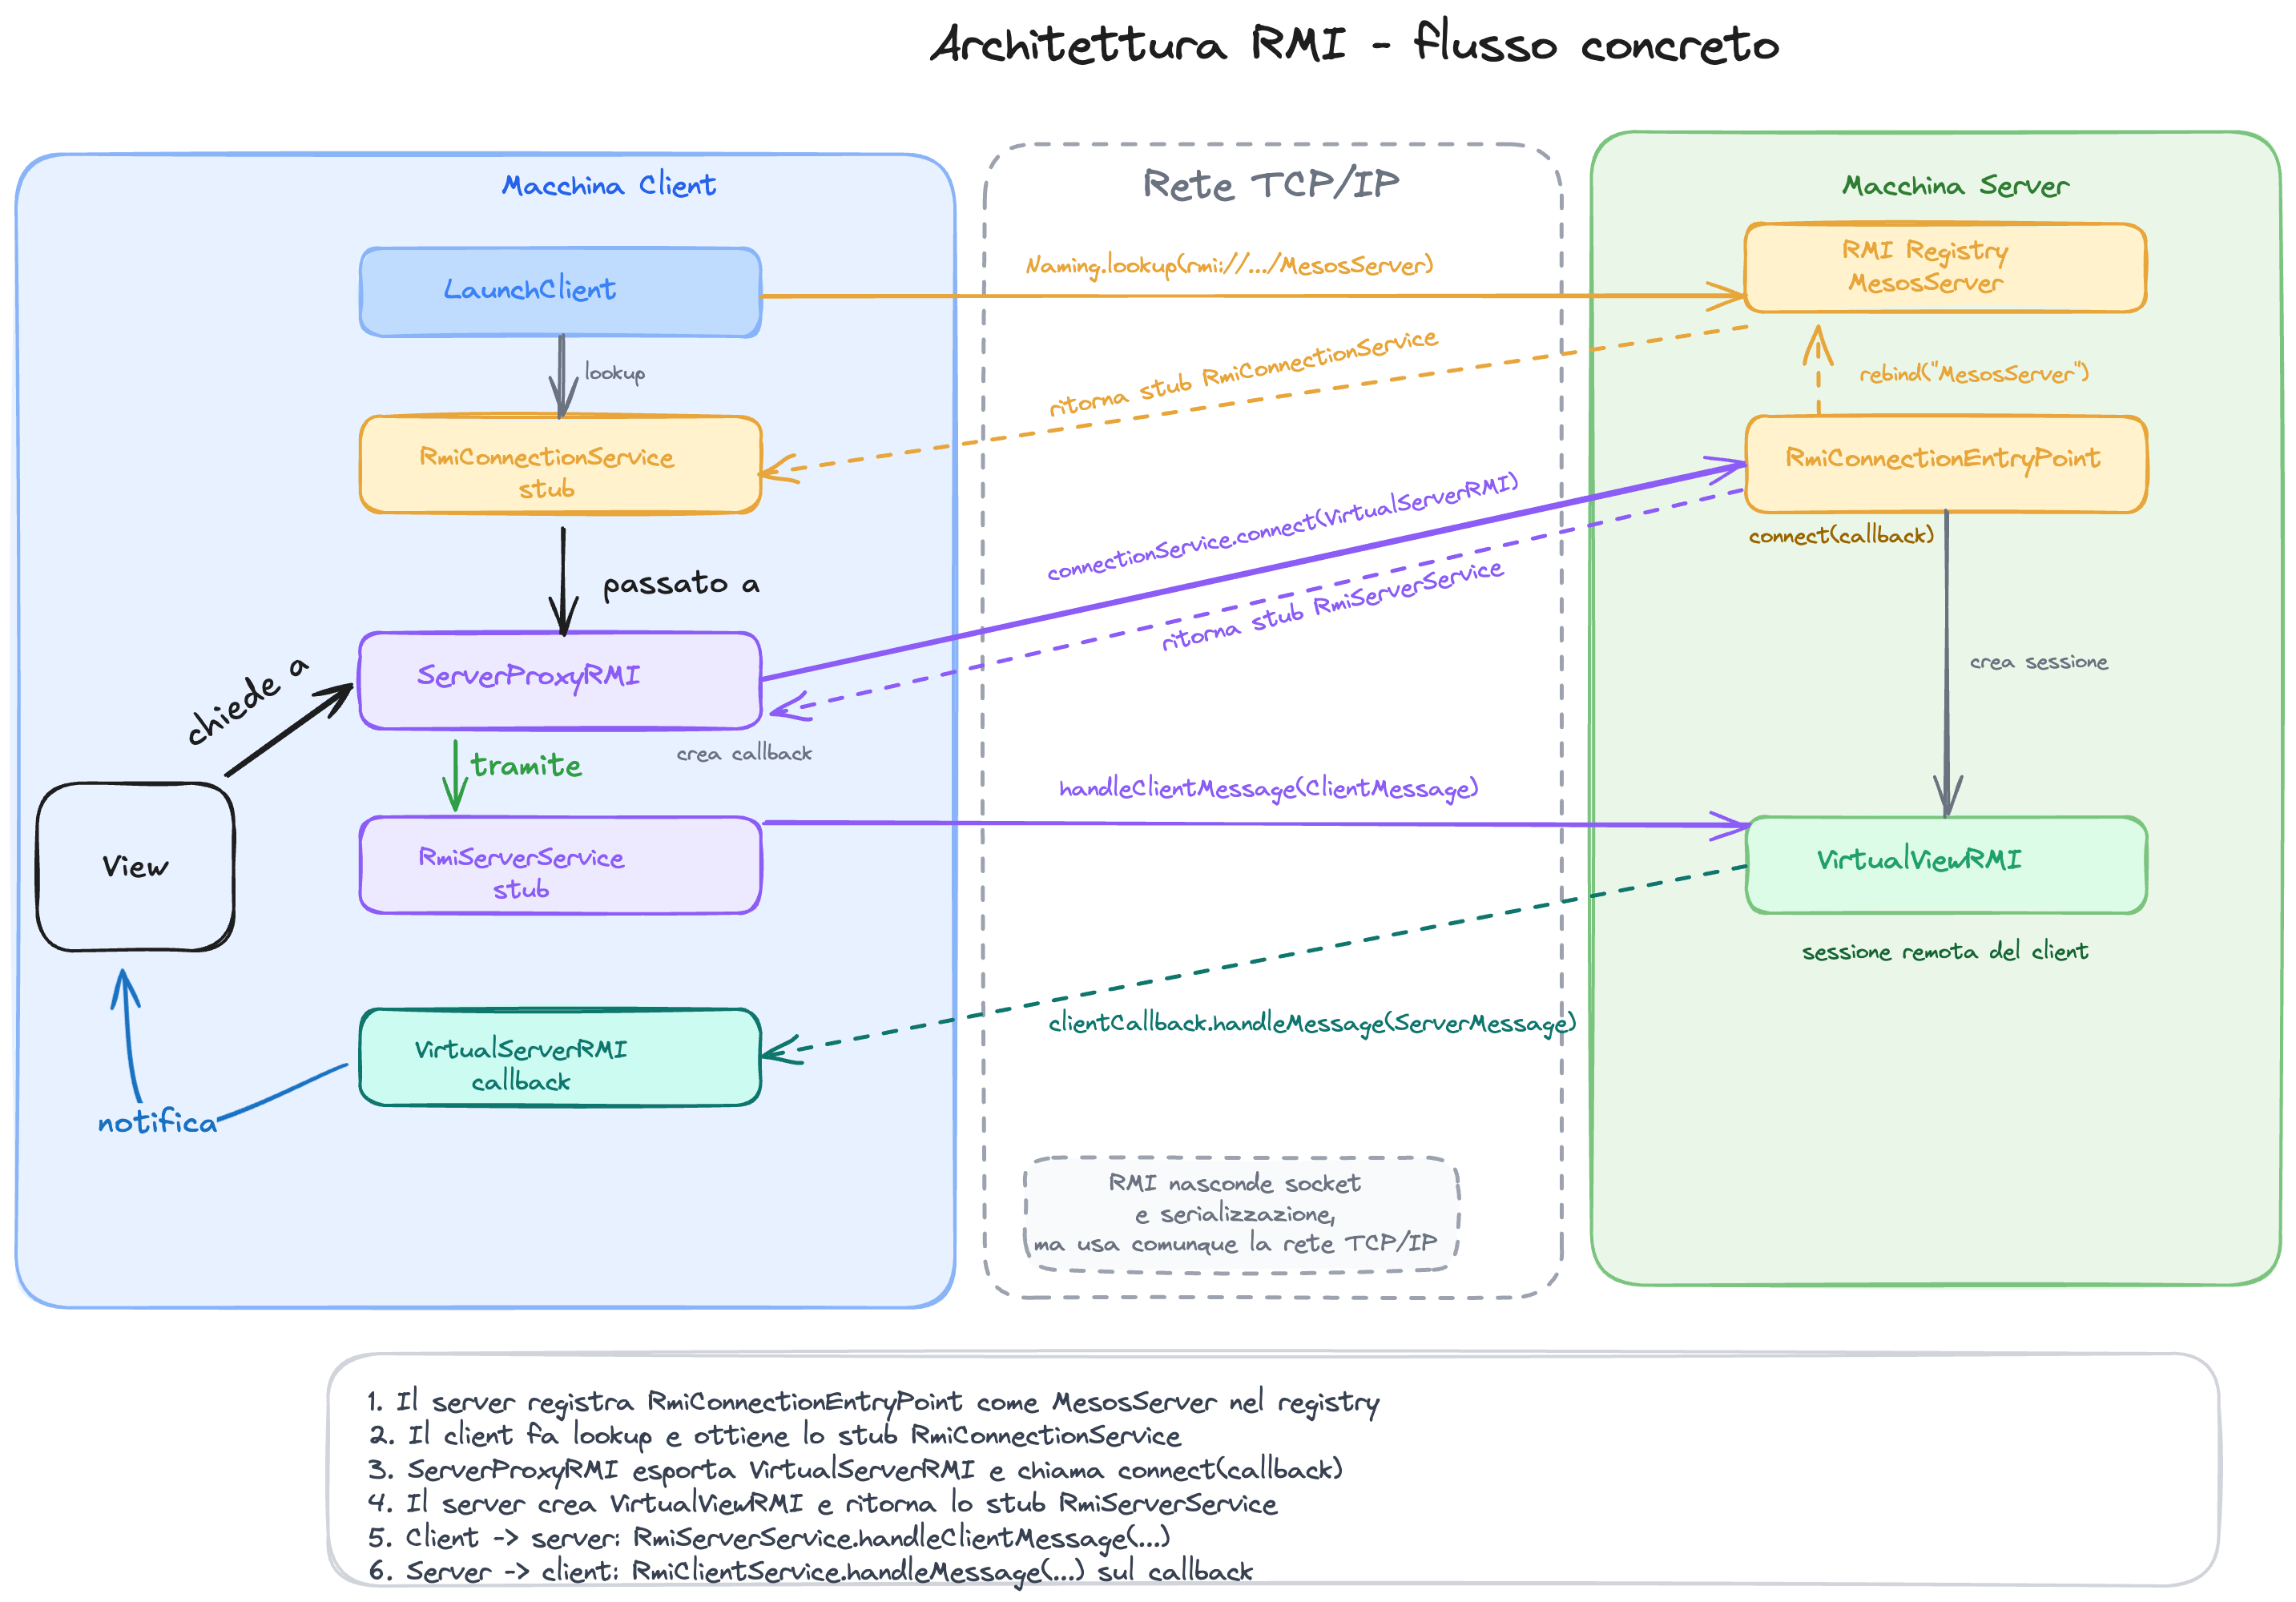
\includegraphics[width=\textwidth]{FlussoRMI.png}
    \caption{Flusso RMI}
\end{figure}

In sintesi il flusso concreto RMI è:
\begin{itemize}
    \item il server registra \texttt{RmiConnectionEntryPoint} nel registry come \texttt{MesosServer};
    \item il client fa lookup e ottiene lo stub \texttt{RmiConnectionService};
    \item il client esporta \texttt{VirtualServerRMI} come callback e chiama \texttt{connect(callback)};
    \item il server crea una \texttt{VirtualViewRMI} dedicata e restituisce lo stub
    \texttt{RmiServerService};
    \item client $\rightarrow$ server: \texttt{ServerProxyRMI} invoca \texttt{VirtualViewRMI}
    tramite stub;
    \item server $\rightarrow$ client: \texttt{VirtualViewRMI} invoca \texttt{VirtualServerRMI}
    tramite callback.
\end{itemize}

\section{Sequence Diagrams Commentati}

In questa sezione vengono commentati alcuni sequence diagram che aiutano a
comprendere il flusso concreto di messaggi tra client e server, sia in TCP che
in RMI.

% ─────────────────────────────────────────────────────────────────────────────
\subsection{Boot: avvio del server e connessione dei client}

Il diagramma mostra le tre fasi dell'avvio del sistema: l'inizializzazione del
server, la connessione di un client TCP e la connessione di un client RMI.

\begin{figure}[H]
    \centering
    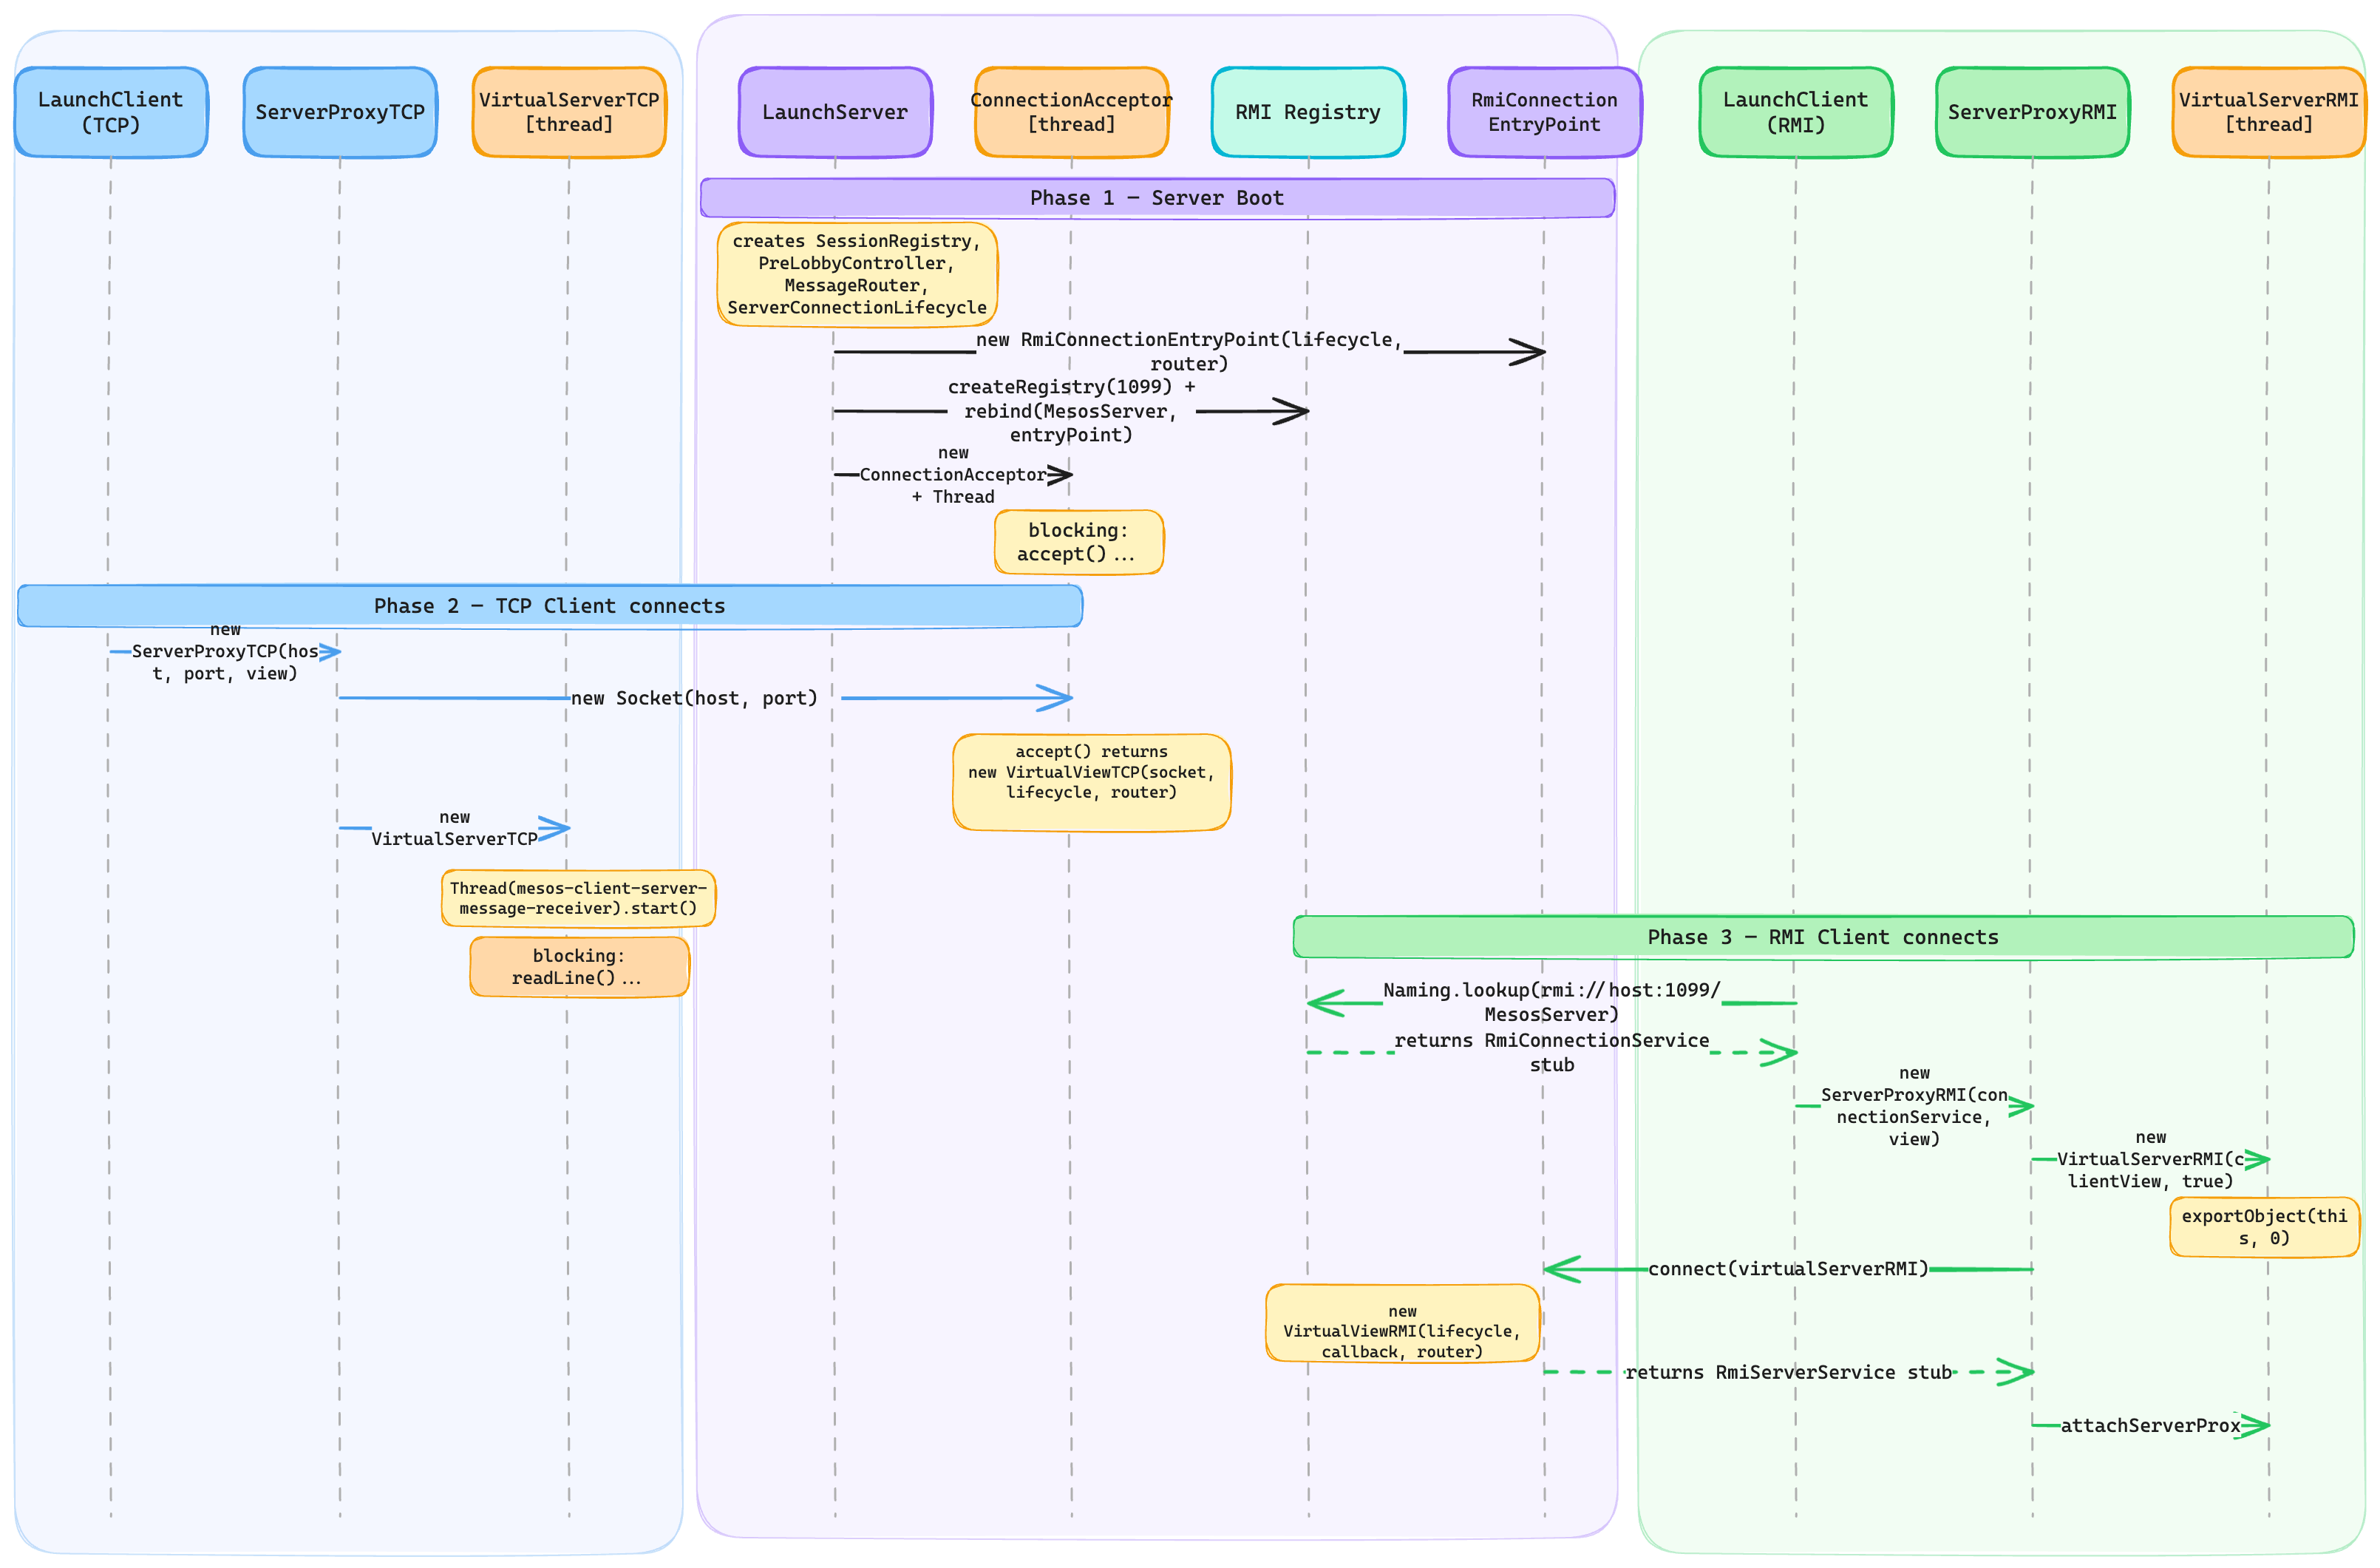
\includegraphics[width=\textwidth]{sequence-boot.png}
    \caption{Sequence diagram — Boot: avvio del server e connessione TCP/RMI}
\end{figure}

\subsubsection*{Fase 1 — Avvio del server (\texttt{LaunchServer})}

\texttt{LaunchServer} inizializza i componenti del server nel seguente ordine:

\begin{enumerate}
    \item Crea \texttt{ServerSessionRegistry}, il registro centralizzato delle
          sessioni di rete, delle lobby e delle partite.

    \item Crea \texttt{PreLobbyController} e lo avvia su un thread dedicato.
          Il controller si mette subito in ascolto sulla sua coda di comandi.

    \item Crea \texttt{MessageRouter} (server-side): il componente che,
          ricevuto un \texttt{ClientPayload}, consulta il registry per
          determinare la fase della sessione e instrada il messaggio al
          controller corretto.

    \item Crea \texttt{ServerConnectionLifecycle}: gestisce gli eventi di
          ingresso e uscita di un client (registrazione, deregistrazione,
          reconnect slot).

    \item Pubblica \texttt{RmiConnectionEntryPoint} nel registry RMI come
          \texttt{MesosServer}. Da questo momento i client RMI possono
          richiedere una connessione.

    \item Avvia \texttt{ConnectionAcceptor} su un thread dedicato
          (\texttt{mesos-connection-acceptor}), che entra in un ciclo
          bloccante su \texttt{serverSocket.accept()}.
\end{enumerate}

\subsubsection*{Fase 2 — Connessione via TCP}

\texttt{LaunchClient(TCP)} crea una nuova istanza di \texttt{ServerProxyTCP},
il cui costruttore coordina tutto l'handshake lato client:

\begin{lstlisting}[language=Java]
this.socket = new Socket(serverHost, port); // TCP handshake
this.writer = new PrintWriter(this.socket.getOutputStream(), true);
this.virtualServer = new VirtualServerTCP(this.socket, clientView, this);
this.virtualServerThread = new Thread(virtualServer,
        "mesos-client-server-message-receiver");
this.virtualServerThread.start();
\end{lstlisting}

Sul server, \texttt{ConnectionAcceptor} sblocca da \texttt{accept()}, crea un
\texttt{VirtualViewTCP} dedicato al client e lo avvia su thread proprio:

\begin{lstlisting}[language=Java]
Socket clientSocket = this.serverSocket.accept();
VirtualViewTCP virtualView = new VirtualViewTCP(
        clientSocket, this.serverConnectionLifecycle, this.router);
new Thread(virtualView,
        "mesos-virtual-view-" + clientSocket.getPort()).start();
\end{lstlisting}

Al termine dell'handshake, per ogni client TCP sono attivi due thread
simmetrici: \texttt{VirtualViewTCP} (server) e \texttt{VirtualServerTCP}
(client), entrambi bloccati su \texttt{readLine()} in attesa di messaggi.

\subsubsection*{Fase 3 — Connessione via RMI}

\texttt{LaunchClient(RMI)} ottiene lo stub di \texttt{RmiConnectionService}
tramite \texttt{Naming.lookup(url)}, poi istanzia \texttt{ServerProxyRMI}.
Il costruttore orchestra la sequenza di setup:

\begin{enumerate}
    \item Crea e pubblica \texttt{VirtualServerRMI} come oggetto remoto (il
          callback che il server userà per rispondere al client).

    \item Chiama \texttt{connect(callback)} su \texttt{RmiConnectionEntryPoint}
          (lato server). Il server crea e restituisce un \texttt{VirtualViewRMI}
          come stub \texttt{RmiServerService}.

    \item Conserva lo stub in \texttt{this.serverStub}: da ora in poi tutti i
          comandi del client passeranno da qui, senza toccare il registry.

    \item Chiama \texttt{attachServerProxy(this)} su \texttt{VirtualServerRMI}
          per completare il collegamento bidirezionale.
\end{enumerate}



% ─────────────────────────────────────────────────────────────────────────────
\subsection{ChooseCard via TCP}

Il diagramma mostra il ciclo completo di un'azione di gioco — la scelta di
una carta — su connessione TCP. Il punto centrale da evidenziare è dove il
\emph{return} della chiamata avviene rispetto alla elaborazione effettiva sul
server.

\begin{figure}[H]
    \centering
    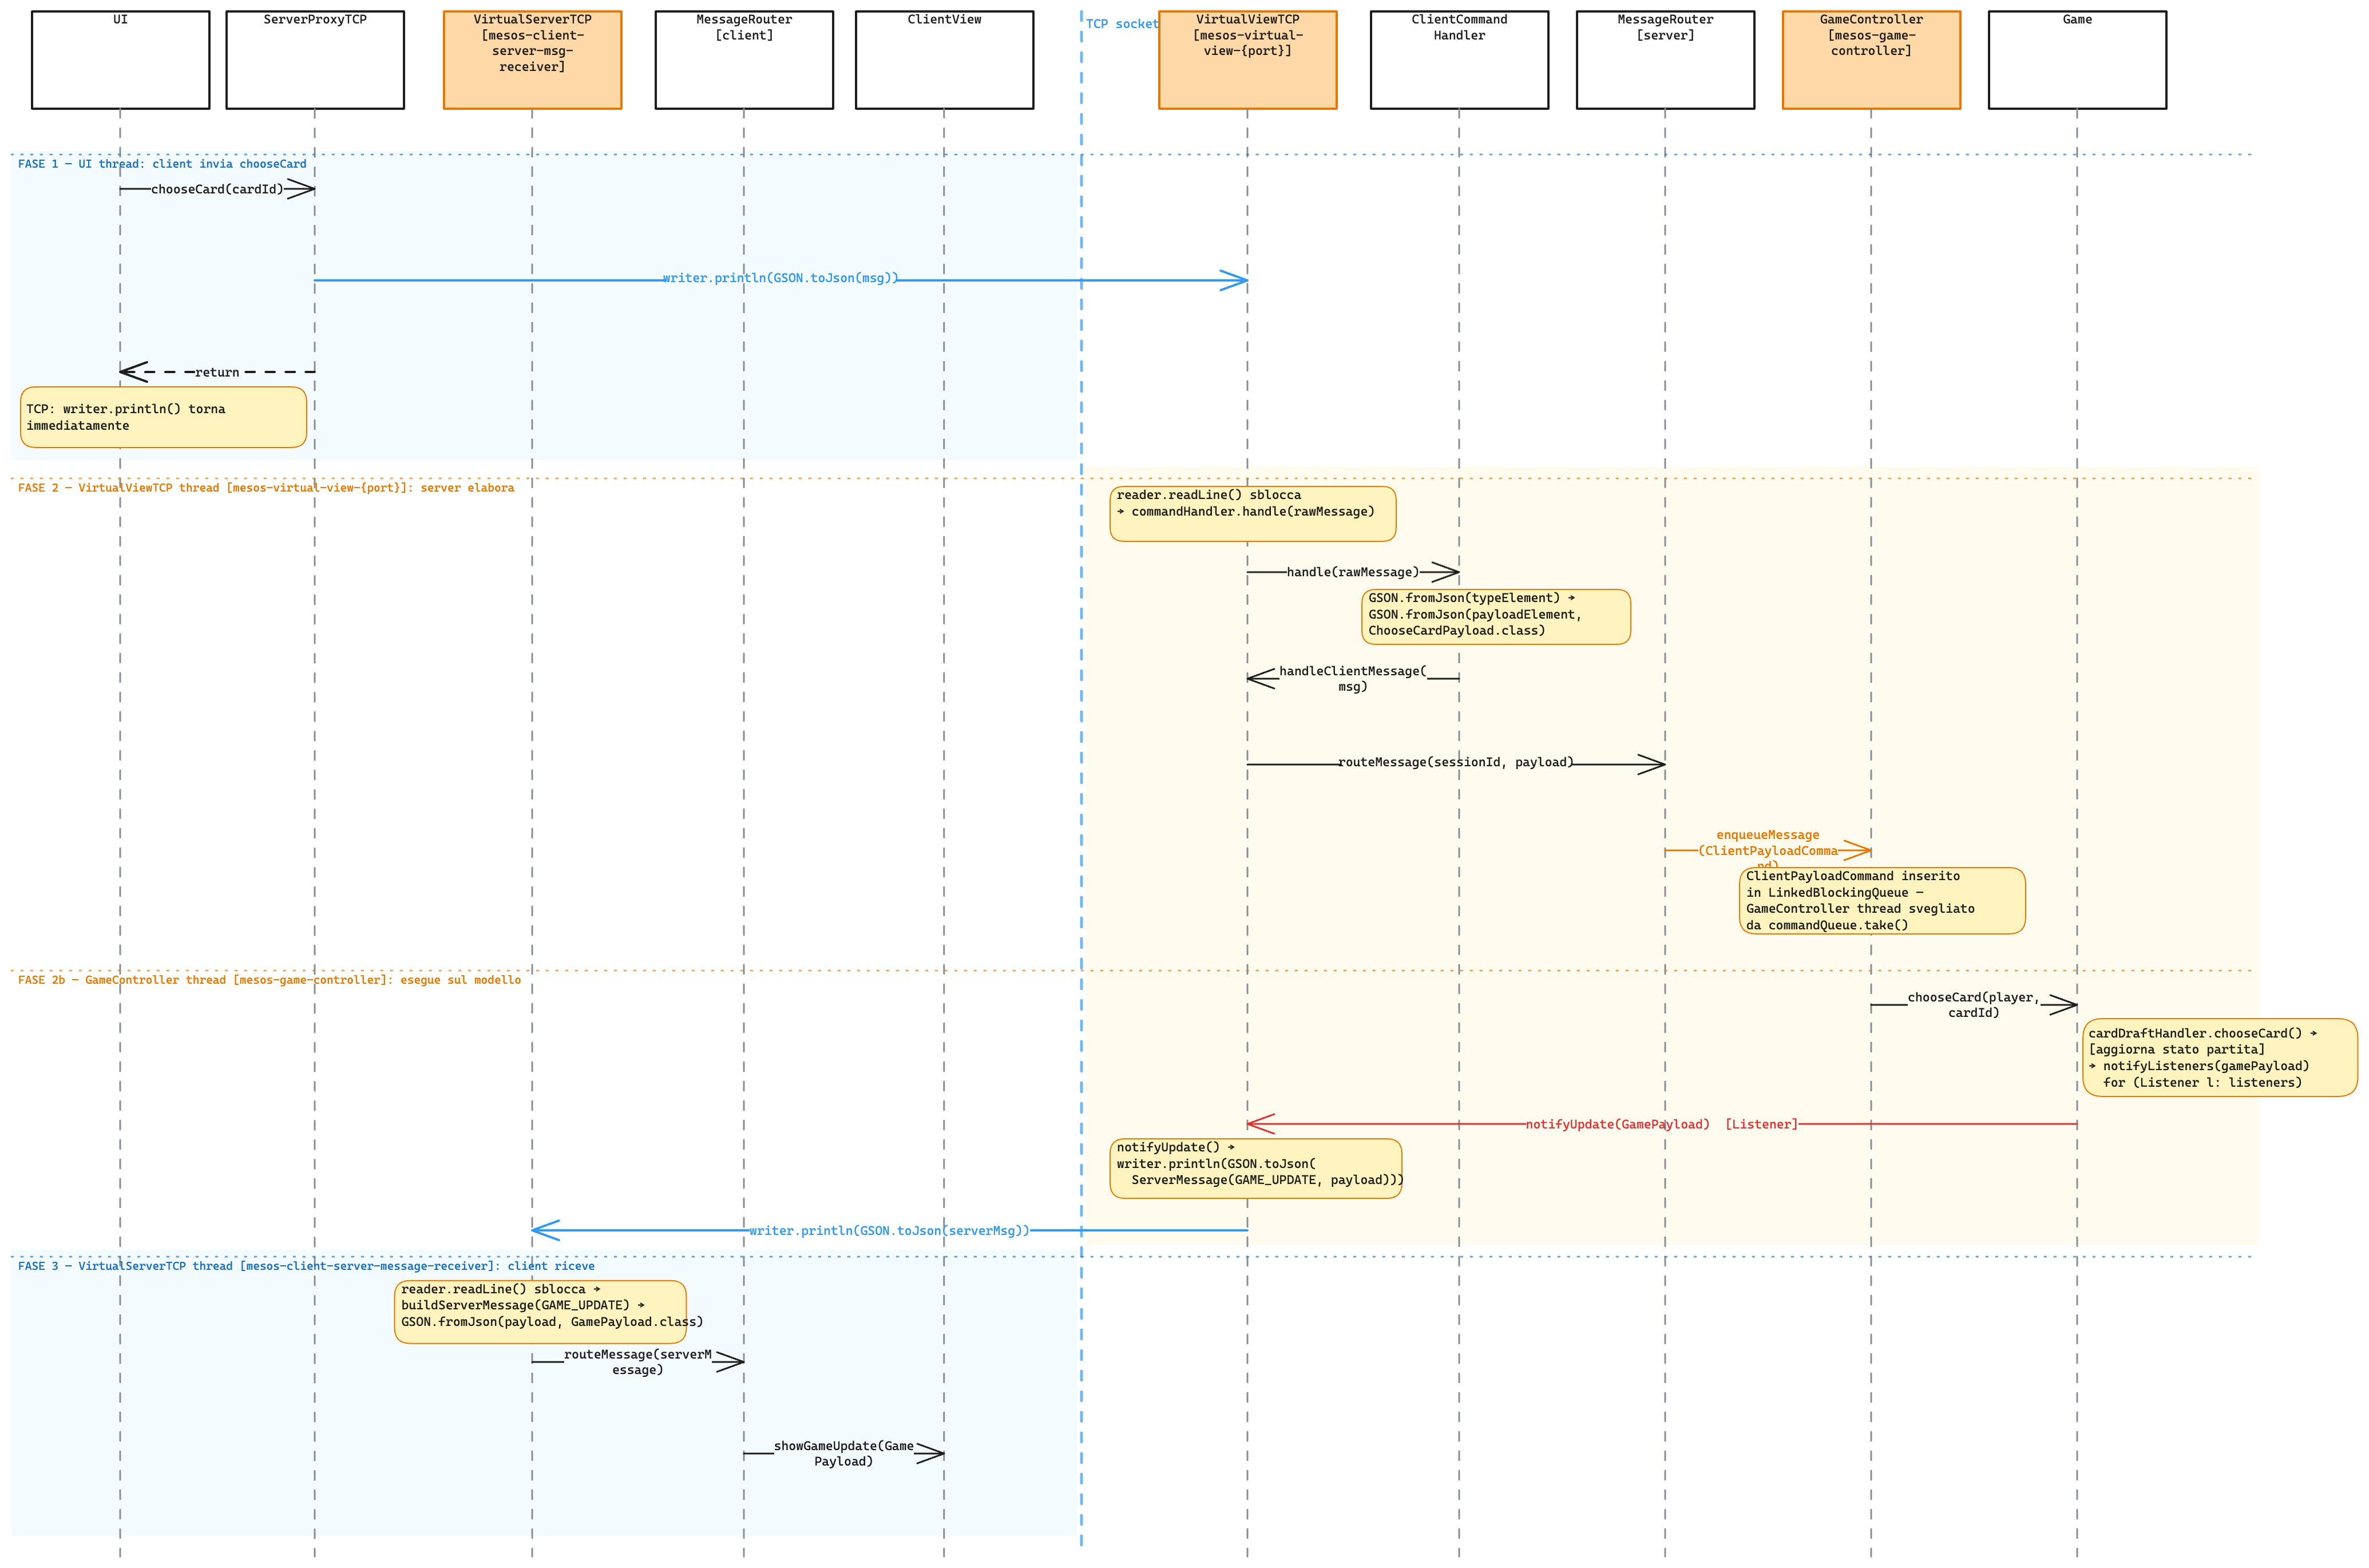
\includegraphics[width=\textwidth]{sequence-choosecard-tcp.png}
    \caption{Sequence diagram — ChooseCard via TCP}
\end{figure}

\subsubsection*{Fase 1 — Invio del comando}

La UI che può essere sia testuale che grafica, chiama \texttt{ServerProxyTCP.chooseCard(cardId)}. Il metodo crea
un \texttt{ChooseCardPayload}, lo insersice in un \texttt{ClientMessage} e
serializza il tutto con GSON:

\begin{lstlisting}[language=Java]
String serialized = GSON.toJson(message);
this.writer.println(serialized); // scrive sul socket e ritorna subito
\end{lstlisting}

\textbf{\texttt{writer.println()} ritorna immediatamente}. 

\subsubsection*{Fase 2 — Elaborazione sul server }

Sul server, il thread \texttt{mesos-virtual-view} era bloccato su
\texttt{reader.readLine()}. Quando il JSON arriva, si sblocca e delega a
\texttt{ClientCommandHandler.handle(rawMessage)}:

\begin{lstlisting}[language=Java]
ClientMessageType type = ClientMessageType.valueOf(typeElement.getAsString());
// ...
ClientPayload payload = GSON.fromJson(payloadElement, ChooseCardPayload.class);
ClientMessage clientMessage = new ClientMessage(type, payload);
this.virtualView.handleClientMessage(clientMessage);
\end{lstlisting}

\texttt{VirtualViewTCP.handleClientMessage()} consegna il payload al
\texttt{MessageRouter} (server-side), che consulta il \texttt{SessionRegistry}
per determinare la fase della sessione (\textsc{game}) e inserisce un
\texttt{ClientPayloadCommand} nella coda del \texttt{GameController}:

\begin{lstlisting}[language=Java]
gameOrchestrator.enqueueMessage(new ClientPayloadCommand(sessionId, payload));
\end{lstlisting}

A questo punto il thread di \texttt{VirtualViewTCP} ha finito: la
\texttt{enqueueMessage} è non bloccante (torna subito) e il thread torna in
attesa della prossima riga sul socket.

Il thread \texttt{mesos-game-controller} era bloccato su
\texttt{commandQueue.take()}. Sbloccato, estrae il comando, risolve il
\texttt{Player} dalla sessione e delega al modello:

\begin{lstlisting}[language=Java]
this.game.chooseCard(player, p.cardId);
\end{lstlisting}

\subsubsection*{Fase 2b — Notifica via Observer (\texttt{Listener})}

Dopo aver aggiornato lo stato, \texttt{Game} chiama \texttt{notifyListeners()}:

\begin{lstlisting}[language=Java]
for (Listener listener : new ArrayList<>(this.listeners)) {
    listener.notifyUpdate(payload);
}
\end{lstlisting}

Ogni \texttt{VirtualViewTCP} è registrato come \texttt{Listener}. La sua
implementazione serializza il payload e scrive sul socket in direzione
server$\rightarrow$client:

\begin{lstlisting}[language=Java]
// VirtualViewTCP.notifyUpdate()
this.writer.println(GSON.toJson(
        new ServerMessage(ServerMessageType.GAME_UPDATE, gamePayload)));
\end{lstlisting}

\subsubsection*{Fase 3 — Ricezione della risposta (client receiver thread)}

Sul client, il thread \texttt{mesos-client-server-message-receiver} era
bloccato su \texttt{reader.readLine()}. Sbloccato, \texttt{VirtualServerTCP}
deserializza il \texttt{ServerMessage} e lo passa al \texttt{MessageRouter}
(client-side):

\begin{lstlisting}[language=Java]
// buildServerMessage() seleziona la classe concreta dal type
GamePayload gamePayload = GSON.fromJson(payload, GamePayload.class);
ServerMessage message = new ServerMessage(type, gamePayload);
this.messageRouter.routeMessage(message);
\end{lstlisting}

Il \texttt{MessageRouter} del client chiama infine
\texttt{clientView.showGameUpdate(gamePayload)}, che aggiorna l'interfaccia
utente. 
\newpage
% ─────────────────────────────────────────────────────────────────────────────
\subsection{ChooseCard via RMI}

Il diagramma mostra lo stesso ciclo di \texttt{chooseCard},
questa volta su connessione RMI. Mette in evidenza le differenze strutturali
rispetto al caso TCP.

\begin{figure}[H]
    \centering
    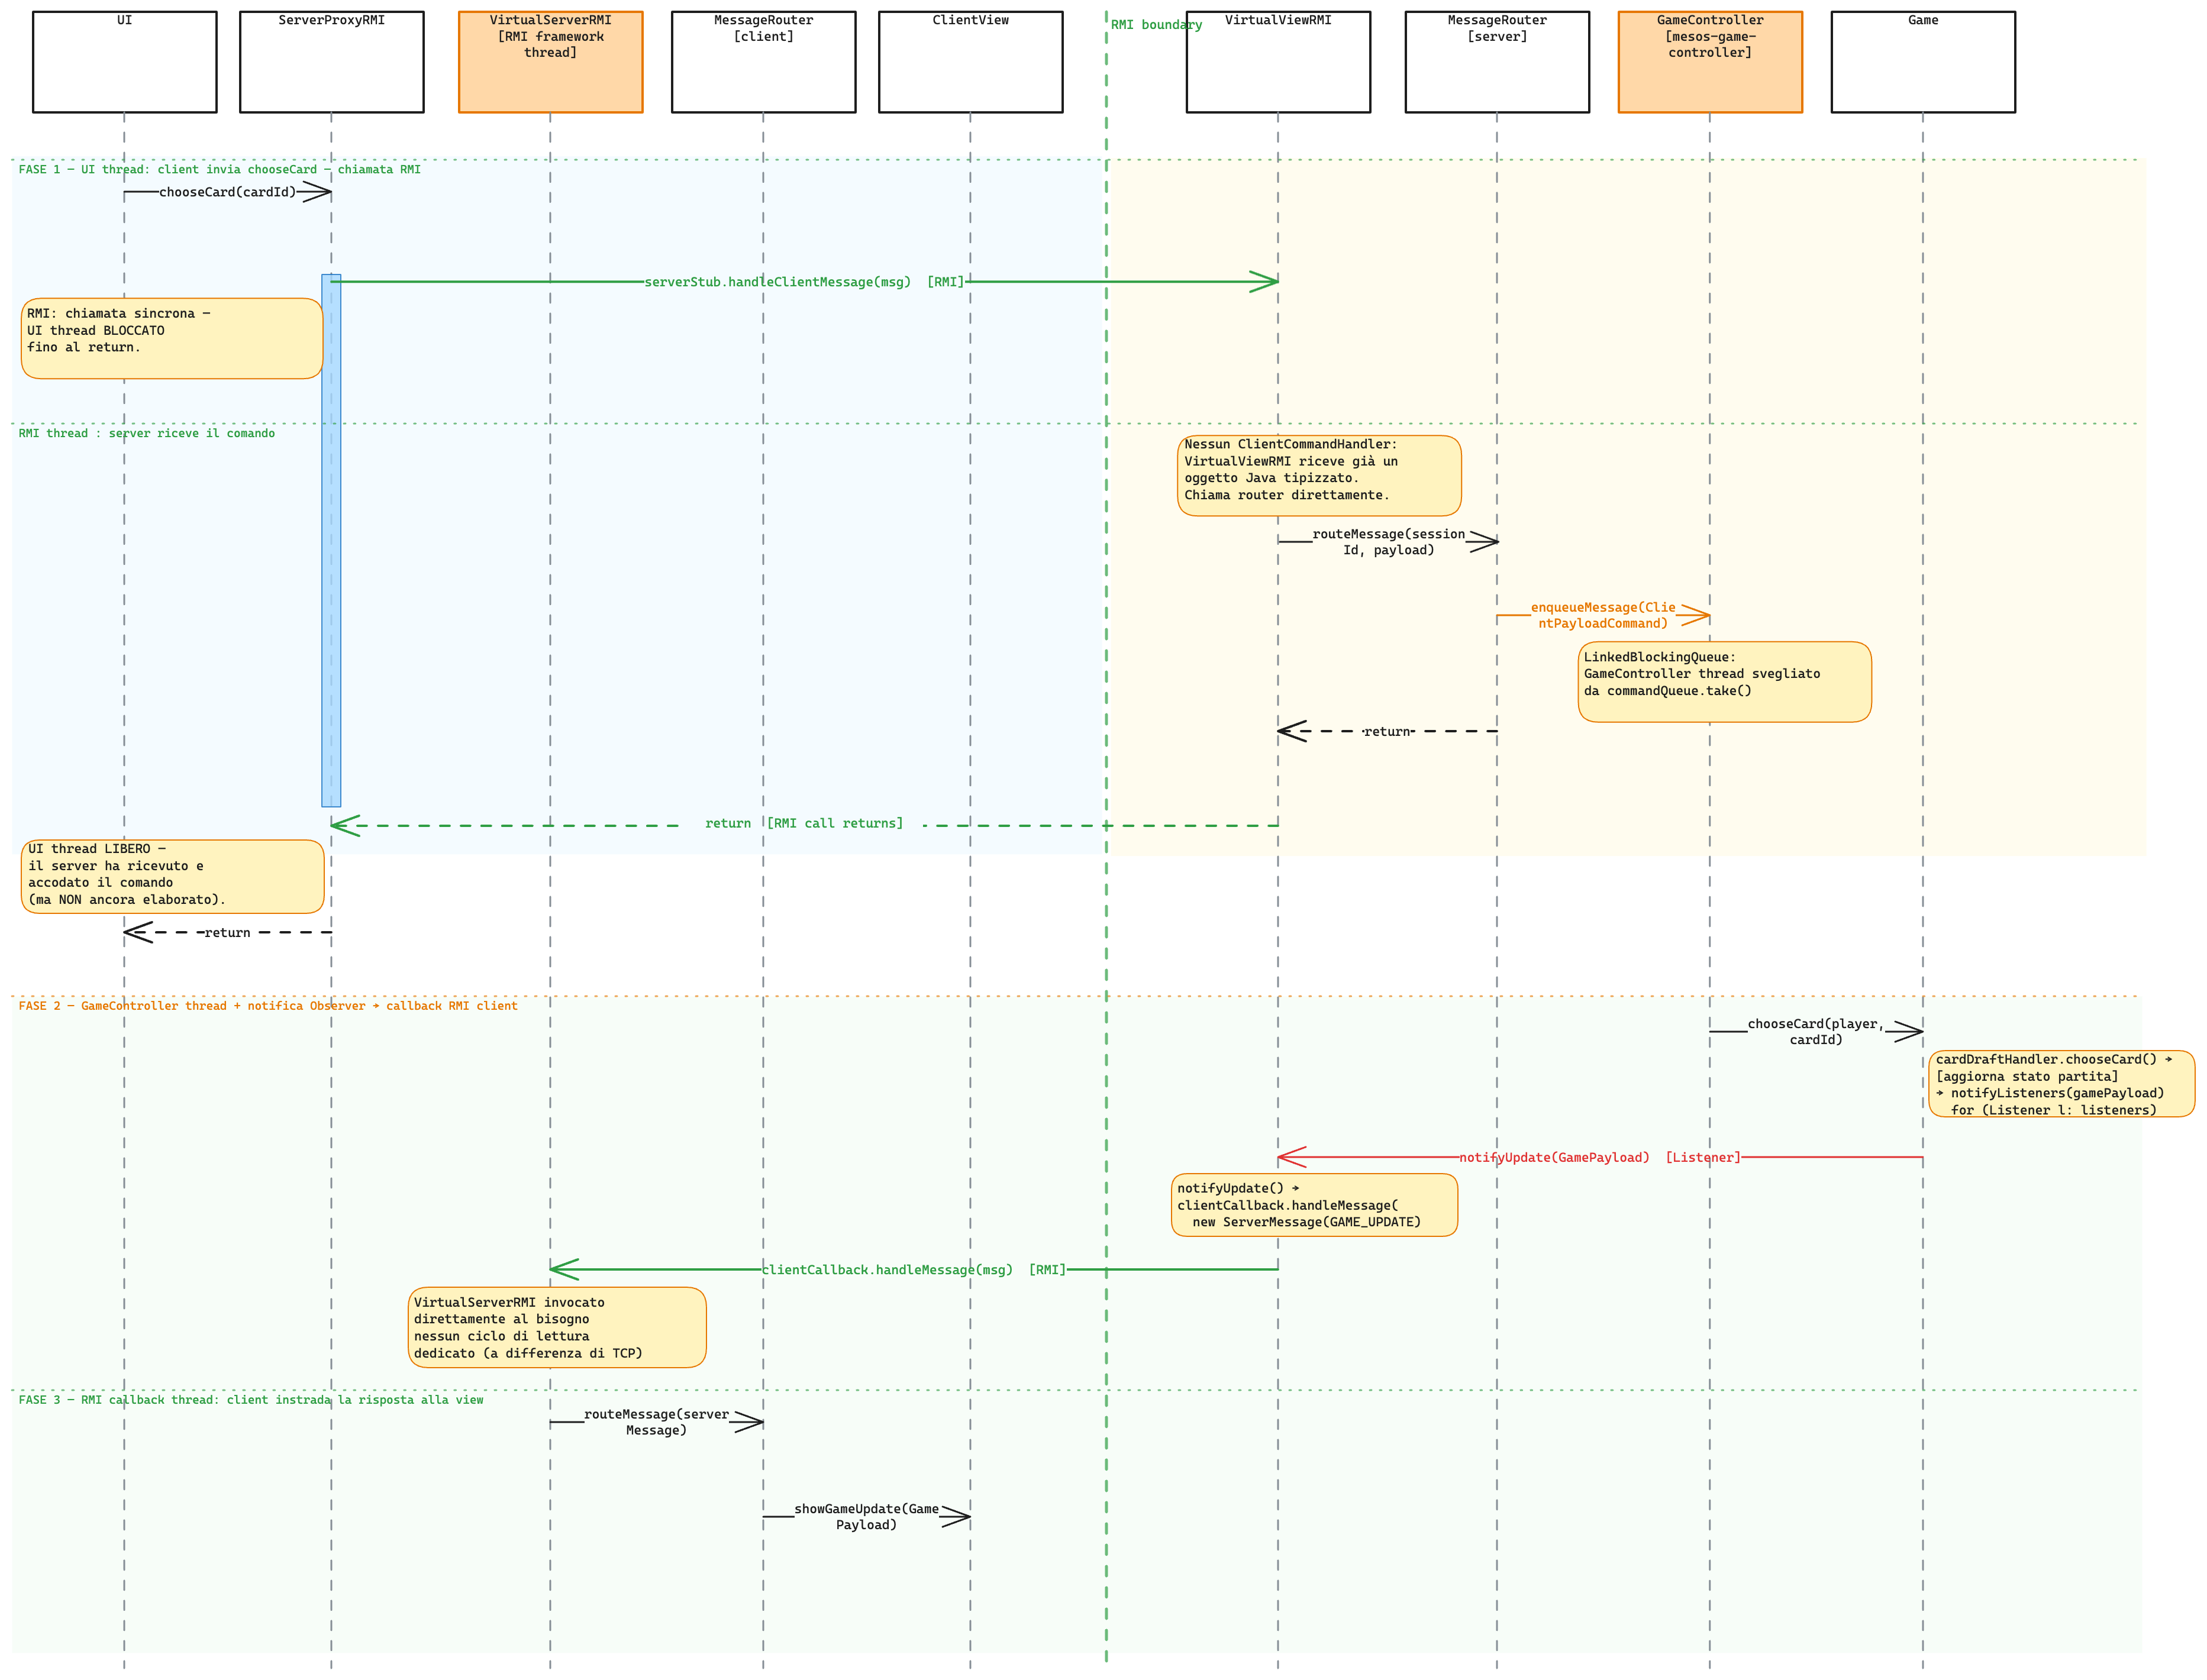
\includegraphics[width=\textwidth]{sequence-choosecard-rmi.png}
    \caption{Sequence diagram — ChooseCard via RMI}
\end{figure}

In questo sequence diagram si può apprezzare come l'implementazione dei controller
su thread con raccolta dei comandi da coda, ci aiuti sensibilmente nel ridurre il gap di 
latenza tra RMI e TCP. Difatti il metodo che inoltra il comando a partire su TCP termina quasi subito,
come si vedrà non è lo stesso per RMI, dove abbiamo che il metodo non torna fintanto che il 
server non ha ricevuto e accodato il comando.

\subsubsection*{Fase 1 — Invio del comando}

La UI chiama \texttt{ServerProxyRMI.chooseCard(cardId)}. Il metodo
crea un \texttt{ChooseCardPayload}, lo avvolge in un \texttt{ClientMessage} e
invoca il metodo remoto sullo stub:

\begin{lstlisting}[language=Java]
this.serverStub.handleClientMessage(message); 
\end{lstlisting}

A differenza di TCP, questa chiamata \textbf{blocca il thread UI} fino a
quando il metodo sul server non ritorna. Non c'è serializzazione GSON esplicita:
i payload vengono passati come oggetti Java tramite la serializzazione standard
di Java RMI.

\subsubsection*{Fase 1b — Elaborazione lato server}

Sul server, la chiamata arriva direttamente in
\texttt{VirtualViewRMI.handleClientMessage(ClientMessage clientMessage)}.
A differenza del caso TCP, non esiste un \texttt{ClientCommandHandler} che
deserializza la stringa JSON: il messaggio è già un oggetto Java tipizzato.
\texttt{VirtualViewRMI} consegna il payload al \texttt{MessageRouter}
direttamente:

\begin{lstlisting}[language=Java]
// VirtualViewRMI.handleClientMessage()
ClientPayload payload = clientMessage.payload;
this.router.routeMessage(this.sessionId, payload);
\end{lstlisting}

\texttt{MessageRouter} inserisce un \texttt{ClientPayloadCommand} nella coda
del \texttt{GameController}, esattamente come nel caso TCP.
Quando \texttt{routeMessage()} ritorna, anche la chiamata RMI ritorna:
il thread UI sul client si sblocca e \texttt{ServerProxyRMI.chooseCard()}
restituisce il controllo all'UI.

\begin{quote}
    Si noti come il thread UI si sblocca dopo che il server ha
    \emph{ricevuto e accodato} il comando, non dopo che il modello lo ha
    elaborato. Il \texttt{GameController} thread processerà il comando in
    modo asincrono, esattamente come nel caso TCP.
\end{quote}

\subsubsection*{Fase 2 — Elaborazione del modello e notifica}

Il \texttt{GameController} thread processa il comando dalla coda e invoca
\texttt{game.chooseCard(player, cardId)}, identico al caso TCP.
\texttt{Game.notifyListeners()} itera i listener: ogni \texttt{VirtualViewRMI}
registrato riceve \texttt{notifyUpdate(gamePayload)}.

\texttt{VirtualViewRMI.notifyUpdate()} costruisce il \texttt{ServerMessage} e
lo consegna al client tramite il callback remoto:

\begin{lstlisting}[language=Java]
// VirtualViewRMI.notifyUpdate()
this.clientCallback.handleMessage(
        new ServerMessage(ServerMessageType.GAME_UPDATE, gamePayload));
\end{lstlisting}

Questa è un'altra chiamata RMI, ma in direzione inversa: il \emph{server} chiama
un metodo sul \emph{client}.

\subsubsection*{Fase 3 — Ricezione della risposta }

La chiamata arriva in \texttt{VirtualServerRMI.handleMessage(ServerMessage)}.
 Non esiste un ciclo
\texttt{readLine()} come in TCP: il framework RMI gestisce l'arrivo della chiamata remota
in modo trasparente.

\begin{lstlisting}[language=Java]
// VirtualServerRMI.handleMessage()
this.messageRouter.routeMessage(message); // -> clientView.showGameUpdate()
\end{lstlisting}

\bigskip
\noindent\textbf{Tabella comparativa TCP vs RMI (chooseCard):}

\begin{center}
\begin{tabular}{|l|l|l|}
\hline
\textbf{Aspetto} & \textbf{TCP} & \textbf{RMI} \\
\hline
Thread UI dopo invio & libero subito (fire \& forget) & bloccato fino al return \\
Serializzazione & GSON esplicita (JSON su socket) & Java RMI (trasparente) \\
\texttt{ClientCommandHandler} & sì (deserializza JSON) & no (oggetto già tipizzato) \\
Thread di ricezione client & dedicato (\texttt{readLine()} loop) & RMI Library\\
Callback server$\to$client & \texttt{writer.println()} & \texttt{clientCallback.handleMessage()} \\
\hline
\end{tabular}
\end{center}


\end{document}
